\documentclass[UTF8]{article}

\author{H.~Partl}
\title{Minimalism}
\usepackage{amsfonts}
\usepackage{amsmath}
\usepackage{latexsym}
\usepackage{amssymb}
\usepackage{makeidx}

\usepackage{amsmath}
\usepackage{graphicx}

\usepackage{graphicx,graphics,color}
\usepackage{multirow}


\usepackage[compat=1.1.0]{tikz-feynman}

\begin{document}

\section{1}

\subsection{1}

\begin{figure}[hp]
    \centering
    %%%%%%%%%%%%%%%%%%%
    \feynmandiagram [horizontal=a to b] {
    i1 -- [fermion] a -- [fermion] i2,
    a -- [photon] b,
    f1 -- [fermion] b -- [fermion] f2,
    };
    %%%%%%%%%%%%%%%%%%%
    \caption{fig:feynmandiagram.1}
    \label{fig:feynmandiagram.1}
\end{figure}


\begin{figure}[hp]
    \centering
    %%%%%%%%%%%%%%%%%%%
    \feynmandiagram [large, vertical=e to f] {
    a -- [fermion] b -- [photon, momentum=\(k\)] c -- [fermion] d,
    b -- [fermion, momentum'=\(p_{1}\)] e -- [fermion, momentum'=\(p_{2}\)] c,
    e -- [gluon] f,
    h -- [fermion] f -- [fermion] i;
    };
    %%%%%%%%%%%%%%%%%%%
    \caption{fig:feynmandiagram.2}
    \label{fig:feynmandiagram.2}
\end{figure}


\begin{figure}[hp]
    \centering
    %%%%%%%%%%%%%%%%%%%
    \feynmandiagram [horizontal=a to b] {
    i1 [particle=\(e^{-}\)] -- [fermion] a -- [fermion] i2 [particle=\(e^{+}\)],
    a -- [photon, edge label=\(\gamma\), momentum'=\(k\)] b,
    f1 [particle=\(\mu^{+}\)] -- [fermion] b -- [fermion] f2 [particle=\(\mu^{-}\)],
    };
    %%%%%%%%%%%%%%%%%%%
    \caption{fig:feynmandiagram.3}
    \label{fig:feynmandiagram.3}
\end{figure}


\begin{figure}[hp]
    \centering
    %%%%%%%%%%%%%%%%%%%
    \feynmandiagram [horizontal=a to b] {
    i1 [particle=\(e^{-}\)] -- [fermion, very thick] a -- [fermion, opacity=0.2] i2 [particle=\(e^{+}\)],
    a -- [red, photon, edge label=\(\gamma\), momentum'={[arrow style=red]\(k\)}] b,
    f1 [particle=\(\mu^{+}\)] -- [fermion, opacity=0.2] b -- [fermion, very thick] f2 [particle=\(\mu^{-}\)],
    };
    %%%%%%%%%%%%%%%%%%%
    \caption{fig:feynmandiagram.4}
    \label{fig:feynmandiagram.4}
\end{figure}


\begin{figure}[hp]
    \centering
    %%%%%%%%%%%%%%%%%%%
    \feynmandiagram [horizontal=a to b] {
    i1 [particle=\(\tilde W\)] -- [plain, boson] a -- [anti fermion] i2 [particle=\(q\)],
    a -- [charged scalar, edge label=\(\tilde q\)] b,
    f1 [particle=\(\tilde g\)] -- [plain, gluon] b -- [fermion] [particle=\(q\)],
    };
    %%%%%%%%%%%%%%%%%%%
    \caption{fig:feynmandiagram.5}
    \label{fig:feynmandiagram.5}
\end{figure}


\begin{figure}[hp]
    \centering
    %%%%%%%%%%%%%%%%%%%
    % No invisible edge to keep the two photons together
    \feynmandiagram [small, horizontal=a to t1] {
    a [particle=\(\pi^{0}\)] -- [scalar] t1 -- t2 -- t3 -- t1,
    t2 -- [photon] p1 [particle=\(\gamma\)],
    t3 -- [photon] p2 [particle=\(\gamma\)],
    };
    %%%%%%%%%%%%%%%%%%%
    \caption{fig:feynmandiagram.6}
    \label{fig:feynmandiagram.6}
\end{figure}

\begin{figure}[hp]
    \centering
    %%%%%%%%%%%%%%%%%%%
    \feynmandiagram [small, horizontal=a to t1] {
    a [particle=\(\pi^{0}\)] -- [scalar] t1 -- t2 -- t3 -- t1,
    t2 -- [photon] p1 [particle=\(\gamma\)],
    t3 -- [photon] p2 [particle=\(\gamma\)],
    p1 -- [opacity=0.2] p2,
    };
    %%%%%%%%%%%%%%%%%%%
    \caption{fig:feynmandiagram.7}
    \label{fig:feynmandiagram.7}
\end{figure}

% Invisible edge ensures photons are parallel

\begin{figure}[hp]
    \centering
    %%%%%%%%%%%%%%%%%%%
    % Using the default spring layout
    \feynmandiagram [horizontal=a to b] {
    a [particle=\(\mu^{-}\)] -- [fermion] b -- [fermion] f1 [particle=\(\nu_{\mu}\)],
    b -- [boson, edge label=\(W^{-}\)] c,
    f2 [particle=\(\overline \nu_{e}\)] -- [fermion] c -- [fermion] f3 [particle=\(e^{-}\)],
    };
    %%%%%%%%%%%%%%%%%%%
    \caption{fig:feynmandiagram.8}
    \label{fig:feynmandiagram.8}
\end{figure}


\begin{figure}[hp]
    \centering
    %%%%%%%%%%%%%%%%%%%
    % Using the layered layout
    \feynmandiagram [layered layout, horizontal=a to b] {
    a [particle=\(\mu^{-}\)] -- [fermion] b -- [fermion] f1 [particle=\(\nu_{\mu}\)],
    b -- [boson, edge label'=\(W^{-}\)] c,
    c -- [anti fermion] f2 [particle=\(\overline \nu_{e}\)],
    c -- [fermion] f3 [particle=\(e^{-}\)],
    };

    %%%%%%%%%%%%%%%%%%%
    \caption{fig:feynmandiagram.9}
    \label{fig:feynmandiagram.9}
\end{figure}


%the diagram 10:

% Using the layered layout f2--c--f3
% \feynmandiagram [layered layout, horizontal=a to b] {
% a [particle=\(\mu^{-}\)] -- [fermion] b -- [fermion] f1 [particle=\(\nu_{\mu}\)],
% b -- [boson, edge label'=\(W^{-}\)] c,
% f2 -- [anti fermion] c [particle=\(\overline \nu_{e}\)] --
% [fermion] f3 [particle=\(e^{-}\)],
% };

\begin{figure}[hp]
    \centering
    %%%%%%%%%%%%%%%%%%%
    % mannuly decide the drawing process
    \begin{tikzpicture}
        \begin{feynman}
            \vertex (a) {\(\mu^{-}\)};
            \vertex [right=of a] (b);
            \vertex [above right=of b] (f1) {\(\nu_{\mu}\)};
            \vertex [below right=of b] (c);
            \vertex [above right=of c] (f2) {\(\overline \nu_{e}\)};
            \vertex [below right=of c] (f3) {\(e^{-}\)};
            \diagram* {
            (a) -- [fermion] (b) -- [fermion] (f1),
            (b) -- [boson, edge label'=\(W^{-}\)] (c),
            (c) -- [anti fermion] (f2),
            (c) -- [fermion] (f3),
            };
        \end{feynman}
    \end{tikzpicture}
    %%%%%%%%%%%%%%%%%%%
    \caption{fig:feynmandiagram.11}
    \label{fig:feynmandiagram.11}
\end{figure}


\begin{figure}[hp]
    \centering
    %%%%%%%%%%%%%%%%%%%
    \feynmandiagram [nodes=circle, horizontal=a1 to b3] {
    a1 -- {b1, b2, b3 -- {c1, c2 -- d1}}
    };

    %%%%%%%%%%%%%%%%%%%
    \caption{fig:feynmandiagram.12}
    \label{fig:feynmandiagram.12}
\end{figure}

\begin{figure}[hp]
    \centering
    %%%%%%%%%%%%%%%%%%%
    \tikzfeynmanset{every feynman={red}}
    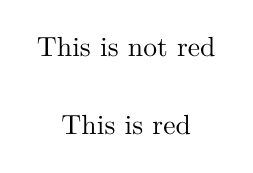
\begin{tikzpicture}
        \node at (0, 0.5) {This is not red};
        \begin{feynman}
            \node at (0, -0.5) {This is red};
        \end{feynman}
    \end{tikzpicture}
    %%%%%%%%%%%%%%%%%%%
    \caption{fig:feynmandiagram.13}
    \label{fig:feynmandiagram.13}
\end{figure}

\begin{figure}[hp]
    \centering
    %%%%%%%%%%%%%%%%%%%
    \begin{equation}
        \feynmandiagram [inline=(d.base), horizontal=d to b] {
        a -- [fermion] b -- [fermion] c,
        b -- [boson] d [particle=\(\gamma\)],
        };
        = i g_{e} \gamma^{\mu}
    \end{equation}

    %%%%%%%%%%%%%%%%%%%
    \caption{fig:feynmandiagram.14}
    \label{fig:feynmandiagram.14}
\end{figure}

\begin{figure}[hp]
    \centering
    %%%%%%%%%%%%%%%%%%%
    \begin{equation}
        \feynmandiagram [baseline=(d.base), horizontal=d to b] {
        a -- [fermion] b -- [fermion] c,
        b -- [boson] d [particle=\(\gamma\)],
        };
        = i g_{e} \gamma^{\mu}
    \end{equation}
    %%%%%%%%%%%%%%%%%%%
    \caption{fig:feynmandiagram.15}
    \label{fig:feynmandiagram.15}
\end{figure}


\begin{figure}[hp]
    \centering
    %%%%%%%%%%%%%%%%%%%
    \feynmandiagram [inline=(b), horizontal=a to b, red] {
    a -- b -- {c [particle=\(c\)], d [particle=\(d\)]}
    };
    \feynmandiagram [inline=(b), horizontal'=a to b, blue] {
    a -- b -- {c [particle=\(c\)], d [particle=\(d\)]}
    };
    \feynmandiagram [inline=(b), vertical=a to b, green!40!black] {
    a -- b -- {c [particle=\(c\)], d [particle=\(d\)]}
    };
    \feynmandiagram [inline=(b), vertical=b to a, black] {
    a -- b -- {c [particle=\(c\)], d [particle=\(d\)]}
    };
    %%%%%%%%%%%%%%%%%%%
    \caption{fig:feynmandiagram.16}
    \label{fig:feynmandiagram.16}
\end{figure}



\begin{figure}[hp]
    \centering
    %%%%%%%%%%%%%%%%%%%
    \tikzfeynmanset{every diagram={red}}
    \feynmandiagram [small, horizontal =d to b] {
    a -- [fermion] b -- [fermion] c,
    b -- [boson] d,
    };
    %%%%%%%%%%%%%%%%%%%
    \caption{fig:feynmandiagram.17}
    \label{fig:feynmandiagram.17}
\end{figure}


\begin{figure}[hp]
    \centering
    %%%%%%%%%%%%%%%%%%%
    \feynmandiagram [baseline=(b), small, horizontal=d to b, red] {
    a -- [fermion] b -- [fermion] c,
    b -- [boson] d,
    };
    \feynmandiagram [baseline=(b), medium, horizontal=d to b, green!40!black] {
    a -- [fermion] b -- [fermion] c,
    b -- [boson] d,
    };
    \feynmandiagram [baseline=(b), large, horizontal=d to b, blue] {
    a -- [fermion] b -- [fermion] c,
    b -- [boson] d,
    };
    %%%%%%%%%%%%%%%%%%%
    \caption{fig:feynmandiagram.18}
    \label{fig:feynmandiagram.18}
\end{figure}

\begin{figure}[hp]
    \centering
    %%%%%%%%%%%%%%%%%%%
    /graph drawing/spring layout= <string> (no default)

    \feynmandiagram [nodes=circle, small, horizontal=c to d] {
    {a, b} -- c -- d -- {e, f},
    };
    %%%%%%%%%%%%%%%%%%%
    \caption{fig:feynmandiagram.19}
    \label{fig:feynmandiagram.19}
\end{figure}

/graph drawing/spring layout= <string> (no default)

\begin{figure}[hp]
    \centering
    %%%%%%%%%%%%%%%%%%%
    \feynmandiagram [nodes=circle,
    small, horizontal=c to d,
    spring electrical layout
    ] {
    {a, b [electric charge=2]} -- c -- d -- {e, f [electric charge=0.1]},
    };
    %%%%%%%%%%%%%%%%%%%
    \caption{fig:feynmandiagram.20}
    \label{fig:feynmandiagram.20}
\end{figure}

\begin{figure}[hp]
    \centering
    %%%%%%%%%%%%%%%%%%%
    \feynmandiagram [nodes=circle, small, horizontal=a to b, layered layout] {
    a -- b -- {c, d -- {e, f}},
    };
    %%%%%%%%%%%%%%%%%%%
    \caption{fig:feynmandiagram.21}
    \label{fig:feynmandiagram.21}
\end{figure}

\begin{figure}[hp]
    \centering
    %%%%%%%%%%%%%%%%%%%
    \feynmandiagram [nodes=circle, small, horizontal=a to b, layered layout] {
    a -- b -- {c -- {c1, c2}, d -- {d1, d2}},
    {[same layer] c1, d},
    };
    %%%%%%%%%%%%%%%%%%%
    \caption{fig:feynmandiagram.22}
    \label{fig:feynmandiagram.22}
\end{figure}


\begin{figure}[hp]
    \centering
    %%%%%%%%%%%%%%%%%%%
    \feynmandiagram [nodes=circle, small, horizontal=a to b, tree layout] {
    a -- b -- {c, d -- {e, f}},
    };
    %%%%%%%%%%%%%%%%%%%
    \caption{fig:feynmandiagram.23}
    \label{fig:feynmandiagram.23}
\end{figure}


\begin{figure}[hp]
    \centering
    %%%%%%%%%%%%%%%%%%%
    \feynmandiagram [nodes=circle, small, horizontal=a to b, tree layout] {
    a -- b -- {c -- {c1, c2}, d -- {d1, d2}},
    };
    %%%%%%%%%%%%%%%%%%%
    \caption{fig:feynmandiagram.24}
    \label{fig:feynmandiagram.24}
\end{figure}

\begin{figure}[hp]
    \centering
    %%%%%%%%%%%%%%%%%%%
    \tikzfeynmanset{
        every vertex={red, dot},
        every particle={blue},
        every blob={draw=green!40!black, pattern color=green!40!black},
    }
    \feynmandiagram [horizontal=a to b] {
    a [particle={\(\gamma, Z\)}] -- [boson] b [blob],
    c -- [fermion] b -- [fermion] d,
    };
    %%%%%%%%%%%%%%%%%%%
    \caption{fig:feynmandiagram.25}
    \label{fig:feynmandiagram.25}
\end{figure}

\begin{figure}[hp]
    \centering
    %%%%%%%%%%%%%%%%%%%
    \feynmandiagram [small] {
    a -- b [dot] -- {c, d}
    };
    %%%%%%%%%%%%%%%%%%%
    \caption{fig:feynmandiagram.26}
    \label{fig:feynmandiagram.26}
\end{figure}

Modifies the vertex so that it has a small filled square.

\begin{figure}[hp]
    \centering
    %%%%%%%%%%%%%%%%%%%
    \feynmandiagram [small] {
    a -- b [square dot] -- {c, d}
    };
    %%%%%%%%%%%%%%%%%%%
    \caption{fig:feynmandiagram.27}
    \label{fig:feynmandiagram.27}
\end{figure}

Modifies the vertex so that it has a small empty circle.

\begin{figure}[hp]
    \centering
    %%%%%%%%%%%%%%%%%%%
    \feynmandiagram [small] {
    a -- b [empty dot] -- {c, d}
    };
    %%%%%%%%%%%%%%%%%%%
    \caption{fig:feynmandiagram.28}
    \label{fig:feynmandiagram.28}
\end{figure}

Modifies the vertex so that it has a small circle with a cross inside.


\begin{figure}[hp]
    \centering
    %%%%%%%%%%%%%%%%%%%
    \feynmandiagram [small] {
    a -- b [crossed dot] -- {c, d}
    };
    %%%%%%%%%%%%%%%%%%%
    \caption{fig:feynmandiagram.29}
    \label{fig:feynmandiagram.29}
\end{figure}

Modifies the vertex so that it is a large blob, usually used to denote an effective operator.

\begin{figure}[hp]
    \centering
    %%%%%%%%%%%%%%%%%%%
    \feynmandiagram [small] {
    a -- b [blob] -- {c, d}
    };
    %%%%%%%%%%%%%%%%%%%
    \caption{fig:feynmandiagram.30}
    \label{fig:feynmandiagram.30}
\end{figure}

\begin{figure}[hp]
    \centering
    %%%%%%%%%%%%%%%%%%%
    \feynmandiagram [small, horizontal=a to b] {
    a [particle={\(\gamma, Z\)}] -- [boson] b -- {c, d},
    };
    %%%%%%%%%%%%%%%%%%%
    \caption{fig:feynmandiagram.31}
    \label{fig:feynmandiagram.31}
\end{figure}


\subsubsection{Edge Keys}


\begin{figure}[hp]
    \centering
    %%%%%%%%%%%%%%%%%%%
    \tikzfeynmanset{
        every edge={green},
        every boson={red},
        every photon={blue},
    }
    \feynmandiagram [small] {
    a [particle=\(a\)] -- [boson] o -- [photon] b [particle=\(b\)],
    f1 [particle=\(c\)] -- [fermion] o -- [scalar] f2 [particle=\(d\)],
    };
    %%%%%%%%%%%%%%%%%%%
    \caption{fig:feynmandiagram.32}
    \label{fig:feynmandiagram.32}
\end{figure}


\begin{figure}[hp]
    \centering
    %%%%%%%%%%%%%%%%%%%
    \feynmandiagram [horizontal=a to b] {a -- [plain] b};
    \feynmandiagram [horizontal=a to b] {a -- [plain, gluon] b};
    %%%%%%%%%%%%%%%%%%%
    \caption{fig:feynmandiagram.33}
    \label{fig:feynmandiagram.33}
\end{figure}



\begin{figure}[hp]
    \centering
    %%%%%%%%%%%%%%%%%%%
    \feynmandiagram [horizontal=a to b] {a -- [boson] b};
    %%%%%%%%%%%%%%%%%%%
    \caption{fig:feynmandiagram.34}
    \label{fig:feynmandiagram.34}
\end{figure}

Draws a sinusoidal line with an arrow to denote a charged boson.

\begin{figure}[hp]
    \centering
    %%%%%%%%%%%%%%%%%%%
    \feynmandiagram [horizontal=a to b] {a -- [charged boson] b};
    %%%%%%%%%%%%%%%%%%%
    \caption{fig:feynmandiagram.35}
    \label{fig:feynmandiagram.35}
\end{figure}


Draws a sinusoidal line with an arrow pointing the other way to to denote a anti charged boson.

\begin{figure}[hp]
    \centering
    %%%%%%%%%%%%%%%%%%%
    \feynmandiagram [horizontal=a to b] {a -- [anti charged boson] b};
    %%%%%%%%%%%%%%%%%%%
    \caption{fig:feynmandiagram.36}
    \label{fig:feynmandiagram.36}
\end{figure}


Draws a sinusoidal line to denote a photon.

\begin{figure}[hp]
    \centering
    %%%%%%%%%%%%%%%%%%%
    \feynmandiagram [horizontal=a to b] {a -- [photon] b};
    %%%%%%%%%%%%%%%%%%%
    \caption{fig:feynmandiagram.37}
    \label{fig:feynmandiagram.37}
\end{figure}

Draws a dashed line to denote a scalar.

\begin{figure}[hp]
    \centering
    %%%%%%%%%%%%%%%%%%%
    \feynmandiagram [horizontal=a to b] {a -- [scalar] b};
    %%%%%%%%%%%%%%%%%%%
    \caption{fig:feynmandiagram.38}
    \label{fig:feynmandiagram.38}
\end{figure}

Draws a dashed line with an arrow to denote a charged scalar.

\begin{figure}[hp]
    \centering
    %%%%%%%%%%%%%%%%%%%
    \feynmandiagram [horizontal=a to b] {a -- [charged scalar] b};
    %%%%%%%%%%%%%%%%%%%
    \caption{fig:feynmandiagram.39}
    \label{fig:feynmandiagram.39}
\end{figure}

Draws a dashed line with an arrow pointing the other way to denote a charged scalar antiparticle.

\begin{figure}[hp]
    \centering
    %%%%%%%%%%%%%%%%%%%
    \feynmandiagram [horizontal=a to b] {a -- [anti charged scalar] b};
    %%%%%%%%%%%%%%%%%%%
    \caption{fig:feynmandiagram.40}
    \label{fig:feynmandiagram.40}
\end{figure}

Draws a dotted line to denote a ghost.

\begin{figure}[hp]
    \centering
    %%%%%%%%%%%%%%%%%%%
    \feynmandiagram [horizontal=a to b] {a -- [ghost] b};
    %%%%%%%%%%%%%%%%%%%
    \caption{fig:feynmandiagram.41}
    \label{fig:feynmandiagram.41}
\end{figure}

Draws a solid line with an arrow pointing the other way to denote an antifermion.

\begin{figure}[hp]
    \centering
    %%%%%%%%%%%%%%%%%%%
    \feynmandiagram [horizontal=a to b] {a -- [anti fermion] b};
    %%%%%%%%%%%%%%%%%%%
    \caption{fig:feynmandiagram.42}
    \label{fig:feynmandiagram.42}
\end{figure}

Draws a solid line with two arrows pointing to the center to denote an Majorana particle.

\begin{figure}[hp]
    \centering
    %%%%%%%%%%%%%%%%%%%
    \feynmandiagram [horizontal=a to b] {a -- [majorana] b};
    %%%%%%%%%%%%%%%%%%%
    \caption{fig:feynmandiagram.43}
    \label{fig:feynmandiagram.43}
\end{figure}

Draws a solid line with two arrows pointing to the ends to denote a Majorana particle.

\begin{figure}[hp]
    \centering
    %%%%%%%%%%%%%%%%%%%
    \feynmandiagram [horizontal=a to b] {a -- [anti majorana] b};
    %%%%%%%%%%%%%%%%%%%
    \caption{fig:feynmandiagram.44}
    \label{fig:feynmandiagram.44}
\end{figure}

Draws a coiled line to denote a gluon.

\begin{figure}[hp]
    \centering
    %%%%%%%%%%%%%%%%%%%
    \feynmandiagram [horizontal=a to b] {a -- [gluon] b};
    %%%%%%%%%%%%%%%%%%%
    \caption{fig:feynmandiagram.45}
    \label{fig:feynmandiagram.45}
\end{figure}

Multiple insertions can be placed along a single edge by repeating the style key.
Through the `<options>` argument, the insertion size and style can be changed.

\begin{figure}[hp]
    \centering
    %%%%%%%%%%%%%%%%%%%
    \feynmandiagram [horizontal=a to b] {a -- [insertion=0.33, insertion=0.67] b};
    %%%%%%%%%%%%%%%%%%%
    \caption{fig:feynmandiagram.46}
    \label{fig:feynmandiagram.46}
\end{figure}

Specifies how big the insertion should be. The length of each edge starting from the center will be $\sqrt{2} \times \left< distance \right>$.

\begin{figure}[hp]
    \centering
    %%%%%%%%%%%%%%%%%%%
    \feynmandiagram [horizontal=a to b] {a -- [insertion={[size=10pt]0.4}] b};
    %%%%%%%%%%%%%%%%%%%
    \caption{fig:feynmandiagram.47}
    \label{fig:feynmandiagram.47}
\end{figure}

Specifies additional styles to applying to the lines of the insertion.

\begin{figure}[hp]
    \centering
    %%%%%%%%%%%%%%%%%%%
    \feynmandiagram [horizontal=a to b] {a -- [insertion={[style=red]0.4}] b};
    %%%%%%%%%%%%%%%%%%%
    \caption{fig:feynmandiagram.48}
    \label{fig:feynmandiagram.48}
\end{figure}

\subsubsection{Momentum Keys}


\begin{figure}[hp]
    \centering
    %%%%%%%%%%%%%%%%%%%
    \feynmandiagram [layered layout, horizontal=a to b] {
    a -- [red, fermion, edge label'=\(ab\), momentum={[arrow style=red]\(p_{ab}\)}] b
    -- [blue, photon, edge label'=\(bc\)] c
    -- [green!40!black, scalar, momentum=\(p_{cd}\)] d,
    };
    %%%%%%%%%%%%%%%%%%%
    \caption{fig:feynmandiagram.49}
    \label{fig:feynmandiagram.49}
\end{figure}

\begin{figure}[hp]
    \centering
    %%%%%%%%%%%%%%%%%%%
    \feynmandiagram [layered layout, horizontal=a to b] {
    a -- [red, fermion, edge label'=\(ab\), rmomentum={[arrow style=red]\(p_{ab}\)}] b
    -- [blue, photon, edge label'=\(bc\)] c
    -- [green!40!black, scalar, rmomentum=\(p_{cd}\)] d,
    };
    %%%%%%%%%%%%%%%%%%%
    \caption{fig:feynmandiagram.50}
    \label{fig:feynmandiagram.50}
\end{figure}

\begin{figure}[hp]
    \centering
    %%%%%%%%%%%%%%%%%%%
    \feynmandiagram [layered layout, horizontal=b to c] {
    a -- [photon, momentum=\(p\)] b
    -- [fermion, half left, looseness=1.5, momentum=\(k\)] c
    -- [fermion, half left, looseness=1.5, momentum=\(k-p\)] b,
    c -- [photon, momentum=\(p\)] d,
    };
    %%%%%%%%%%%%%%%%%%%
    \caption{fig:feynmandiagram.51}
    \label{fig:feynmandiagram.51}
\end{figure}


\subsubsection{Modifier Keys}

\begin{figure}[hp]
    \centering
    %%%%%%%%%%%%%%%%%%%
    \feynmandiagram [horizontal=a to b] {
    a -- [red, fermion, half left] b -- [blue, fermion, half left] a,
    };
    %%%%%%%%%%%%%%%%%%%
    \caption{fig:feynmandiagram.52}
    \label{fig:feynmandiagram.52}
\end{figure}


\begin{figure}[hp]
    \centering
    %%%%%%%%%%%%%%%%%%%
    \feynmandiagram [horizontal=a to c] {
    a -- [red!0!blue, fermion, quarter left] b
    -- [red!33!blue, fermion, quarter left] c
    -- [red!66!blue, fermion, quarter left] d
    -- [red!100!blue, fermion, quarter left] a,
    };
    %%%%%%%%%%%%%%%%%%%
    \caption{fig:feynmandiagram.53}
    \label{fig:feynmandiagram.53}
\end{figure}


\subsection{Examples-tikz}

Below are a few diagrams which demonstrate how the package can be used in some more practical examples.

\subsubsection{Vertex Rule}

\begin{figure}[hp]
    \centering
    %%%%%%%%%%%%%%%%%%%
    \feynmandiagram [horizontal=a to b] {
    a [particle=\(Z\)] -- [photon, momentum=\(p_{1}\)] b,
    f1 [particle=\(\overline f\)]
    -- [fermion, rmomentum'=\(p_{3}\)] b
    -- [fermion, momentum=\(p_{2}\)] f2 [particle=\(f\)],
    };
    %%%%%%%%%%%%%%%%%%%
    \caption{fig:feynmandiagram.54}
    \label{fig:feynmandiagram.54}
\end{figure}

\subsection{Tree Level Diagrams}

\begin{figure}[hp]
    \centering
    %%%%%%%%%%%%%%%%%%%
    \feynmandiagram [horizontal=a to b] {
    i1 [particle=\(e^{-}\)] -- [fermion] a -- [fermion] i2 [particle=\(e^{+}\)],
    a -- [photon, edge label=\(\gamma\)] b,
    f1 [particle=\(\mu^{-}\)] -- [fermion] b -- [fermion] f2 [particle=\(\mu^{+}\)],
    };
    %%%%%%%%%%%%%%%%%%%
    \caption{fig:feynmandiagram.55}
    \label{fig:feynmandiagram.55}
\end{figure}

\begin{figure}[hp]
    \centering
    %%%%%%%%%%%%%%%%%%%
    \feynmandiagram [vertical'=a to b] {
    i1 [particle=\(e^{-}\)]
    -- [fermion] a
    -- [fermion] f1 [particle=\(e^{-}\)],
    a -- [photon, edge label=\(\gamma\)] b,
    i2 [particle=\(e^{+}\)]
    -- [anti fermion] b
    -- [anti fermion] f2 [particle=\(e^{+}\)],
    };
    %%%%%%%%%%%%%%%%%%%
    \caption{fig:feynmandiagram.56}
    \label{fig:feynmandiagram.56}
\end{figure}


\begin{figure}[hp]
    \centering
    %%%%%%%%%%%%%%%%%%%
    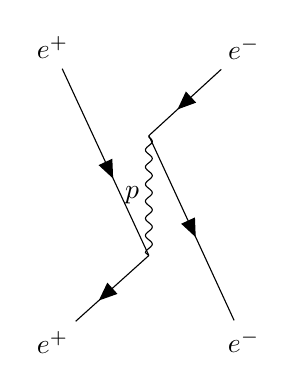
\begin{tikzpicture}
        \begin{feynman}
            \diagram [vertical'=a to b] {
            i1 [particle=\(e^{-}\)]
            -- [fermion] a
            -- [draw=none] f1 [particle=\(e^{+}\)],
            a -- [photon, edge label'=\(p\)] b,
            i2 [particle=\(e^{+}\)]
            -- [anti fermion] b
            -- [draw=none] f2 [particle=\(e^{-}\)],
            };
            \diagram* {
            (a) -- [fermion] (f2),
            (b) -- [anti fermion] (f1),
            };
        \end{feynman}
    \end{tikzpicture}
    %%%%%%%%%%%%%%%%%%%
    \caption{fig:feynmandiagram.57}
    \label{fig:feynmandiagram.57}
\end{figure}

By default, the `\\feynmandiagram' and `\\diagram' commands use the spring layout algorithm to place all the edges. 

%%%%%%%%%%%%%%%%%%%%%%%%%%%%%%%%%%%%%%%%%%%%


\subsection{Loop}

\begin{figure}[hp]
    \centering
    %%%%%%%%%%%%%%%%%%%
    \feynmandiagram [layered layout, horizontal=b to c] {
    a -- [photon, momentum=\(p\)] b
    -- [fermion, half left, momentum=\(k\)] c
    -- [fermion, half left, momentum=\(k-p\)] b,
    c -- [photon, momentum=\(p\)] d,
    };
    %%%%%%%%%%%%%%%%%%%
    \caption{fig:feynmandiagram.58}
    \label{fig:feynmandiagram.58}
\end{figure}

\begin{figure}[hp]
    \centering
    %%%%%%%%%%%%%%%%%%%
    \feynmandiagram [layered layout, horizontal=a to b] [edges=gluon] {
    {i1, i2} -- a -- [half left] b -- [half left] a,
    b -- {f1, f2},
    };
    %%%%%%%%%%%%%%%%%%%
    \caption{fig:feynmandiagram.59}
    \label{fig:feynmandiagram.59}
\end{figure}


\subsection{Box Diagrams}

\begin{figure}[hp]
    \centering
    %%%%%%%%%%%%%%%%%%%
    \feynmandiagram [layered layout, horizontal=a to b] {
    % Draw the top and bottom lines
    i1 [particle=\(d\)]
    -- [fermion] a
    -- [photon, edge label=\(W^{-}\)] b
    -- [fermion] f1 [particle=\(\mu^{-}\)],
    i2 [particle=\(\overline s\)]
    -- [anti fermion] c
    -- [photon, edge label'=\(W^{+}\)] d
    -- [anti fermion] f2 [particle=\(\mu^{+}\)],
    % Draw the two internal fermion lines
    { [same layer] a -- [fermion, edge label'=\(q\)] c },
    { [same layer] b -- [anti fermion, edge label=\(\nu_{\mu}\)] d},
    };
    %%%%%%%%%%%%%%%%%%%
    \caption{fig:feynmandiagram.60}
    \label{fig:feynmandiagram.60}
\end{figure}


\subsection{Meson decay and mixing}

\begin{figure}[hp]
    \centering
    %%%%%%%%%%%%%%%%%%%
    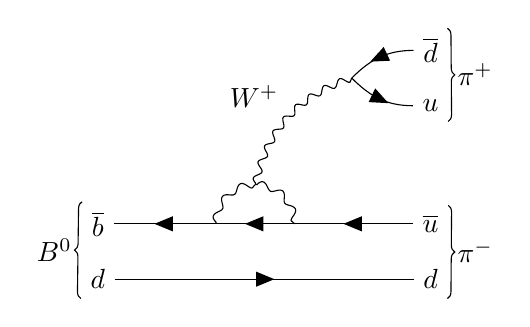
\begin{tikzpicture}
        \begin{feynman}
            \vertex (a1) {\(\overline b\)};
            \vertex[right=1.5cm of a1] (a2);
            \vertex[right=1cm of a2] (a3);
            \vertex[right=1.5cm of a3] (a4) {\(\overline u\)};
            \vertex[below=2em of a1] (b1) {\(d\)};
            \vertex[below=2em of a4] (b2) {\(d\)};
            %% See section 13.5 of PGF/TikZ manual
            \vertex at ($(a2)!0.5!(a3)!0.5cm!90:(a3)$) (d);
            %% Equivalent way to obtain (d):
            % \vertex at ($(b2)!0.5!(b3) + (0, -0.5cm)$) (d);
            \vertex[above=of a4] (c1) {\(u\)};
            \vertex[above=2em of c1] (c3) {\(\overline d\)};
            \vertex at ($(c1)!0.5!(c3) - (1cm, 0)$) (c2);
            \diagram* {
            (a4) -- [fermion] (a3) -- [fermion] (a2) -- [fermion] (a1),
            (b1) -- [fermion] (b2),
            (c3) -- [fermion, out=180, in=45] (c2) -- [fermion, out=-45, in=180] (c1),
            (a2) -- [boson, quarter left] (d) -- [boson, quarter left] (a3),
            (d) -- [boson, bend left, edge label=\(W^{+}\)] (c2),
            };
            \draw [decoration={brace}, decorate] (b1.south west) -- (a1.north west)
            node [pos=0.5, left] {\(B^{0}\)};
            \draw [decoration={brace}, decorate] (c3.north east) -- (c1.south east)
            node [pos=0.5, right] {\(\pi^{+}\)};
            \draw [decoration={brace}, decorate] (a4.north east) -- (b2.south east)
            node [pos=0.5, right] {\(\pi^{-}\)};
        \end{feynman}
    \end{tikzpicture}
    %%%%%%%%%%%%%%%%%%%
    \caption{fig:feynmandiagram.61}
    \label{fig:feynmandiagram.61}
\end{figure}

\begin{figure}[hp]
    \centering
    %%%%%%%%%%%%%%%%%%%
    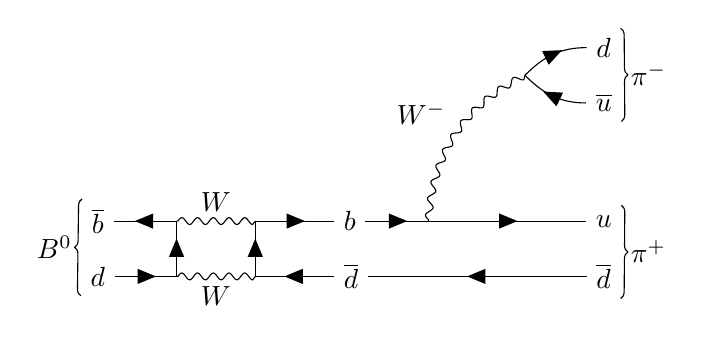
\begin{tikzpicture}
        \begin{feynman}
            \vertex (a1) {\(\overline b\)};
            \vertex[right=1cm of a1] (a2);
            \vertex[right=1cm of a2] (a3);
            \vertex[right=1cm of a3] (a4) {\(b\)};
            \vertex[right=1cm of a4] (a5);
            \vertex[right=2cm of a5] (a6) {\(u\)};
            \vertex[below=2em of a1] (b1) {\(d\)};
            \vertex[right=1cm of b1] (b2);
            \vertex[right=1cm of b2] (b3);
            \vertex[right=1cm of b3] (b4) {\(\overline d\)};
            \vertex[below=2em of a6] (b5) {\(\overline d\)};
            \vertex[above=of a6] (c1) {\(\overline u\)};
            \vertex[above=2em of c1] (c3) {\(d\)};
            \vertex at ($(c1)!0.5!(c3) - (1cm, 0)$) (c2);
            \diagram* {
            {[edges=fermion]
                    (b1) -- (b2) -- (a2) -- (a1),
                    (b5) -- (b4) -- (b3) -- (a3) -- (a4) -- (a5) -- (a6),
                },
            (a2) -- [boson, edge label=\(W\)] (a3),
            (b2) -- [boson, edge label'=\(W\)] (b3),
            (c1) -- [fermion, out=180, in=-45] (c2) -- [fermion, out=45, in=180] (c3),
            (a5) -- [boson, bend left, edge label=\(W^{-}\)] (c2),
            };
            \draw [decoration={brace}, decorate] (b1.south west) -- (a1.north west)
            node [pos=0.5, left] {\(B^{0}\)};
            \draw [decoration={brace}, decorate] (c3.north east) -- (c1.south east)
            node [pos=0.5, right] {\(\pi^{-}\)};
            \draw [decoration={brace}, decorate] (a6.north east) -- (b5.south east)
            node [pos=0.5, right] {\(\pi^{+}\)};
        \end{feynman}
    \end{tikzpicture}
    %%%%%%%%%%%%%%%%%%%
    \caption{fig:feynmandiagram.62}
    \label{fig:feynmandiagram.62}
\end{figure}


\begin{figure}[hp]
    \centering
    %%%%%%%%%%%%%%%%%%%
    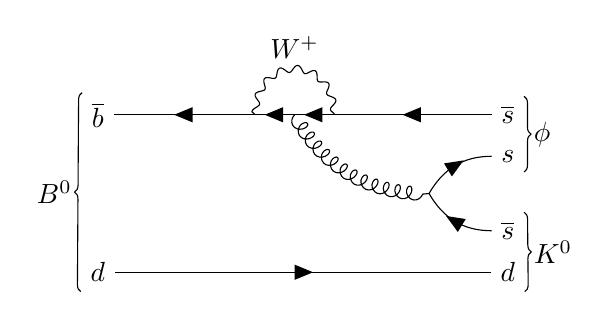
\begin{tikzpicture}
        \begin{feynman}
            \vertex (a1) {\(\overline b\)};
            \vertex[right=2cm of a1] (a2);
            \vertex[right=0.5cm of a2] (a3);
            \vertex[right=0.5cm of a3] (a4);
            \vertex[right=2cm of a4] (a5) {\(\overline s\)};
            \vertex[below=2cm of a1] (b1) {\(d\)};
            \vertex[below=2cm of a5] (b2) {\(d\)};
            \vertex[below=1.5em of a5] (c1) {\(s\)};
            \vertex[above=1.5em of b2] (c3) {\(\overline s\)};
            \vertex at ($(c1)!0.5!(c3) - (1cm, 0)$) (c2);
            \diagram* {
            {[edges=fermion]
                    (a5) -- (a4) -- (a3) -- (a2) -- (a1),
                },
            (b1) -- [fermion] (b2),
            (c3) -- [fermion, out=180, in=-60] (c2) -- [fermion, out=60, in=180] (c1),
            (a3) -- [gluon, bend right] (c2),
            (a4) -- [boson, out=90, in=90, looseness=2.0, edge label'=\(W^{+}\)] (a2)
            };
            \draw [decoration={brace}, decorate] (b1.south west) -- (a1.north west)
            node [pos=0.5, left] {\(B^{0}\)};
            \draw [decoration={brace}, decorate] (a5.north east) -- (c1.south east)
            node [pos=0.5, right] {\(\phi\)};
            \draw [decoration={brace}, decorate] (c3.north east) -- (b2.south east)
            node [pos=0.5, right] {\(K^{0}\)};
        \end{feynman}
    \end{tikzpicture}
    %%%%%%%%%%%%%%%%%%%
    \caption{fig:feynmandiagram.63}
    \label{fig:feynmandiagram.63}
\end{figure}








\end{document}